%!TEX root = ../luanvan.tex
\chapter{Kết quả thực nghiệm}
\section{Môi trường phát triển phần mềm}
\subsection{Phần cứng}

Hệ thống quản lý VBCC sử dụng công nghệ blockchain đã được triển khai thử nghiệm trên máy tính có cấu hình như sau:
\begin{itemize}
\item CPU: Intel(R) Core(TM) i3-10100F 3.00 GHz
\item RAM: 16 GB
\item Hard Disk: 120 GB NVME SSD
\end{itemize}

\subsection{Phần mềm}
\begin{itemize}
\item Hệ điều hành: Windows 10
\item Docker Desktop: phiên bản 4.13.0
\item Môi trường Nodejs: 12.22.12
\item Trình soạn thảo: Visual Studio Code 1.71
\item Các phần mở rộng của Visual Code: IBM Blockchain Flatform
\item Cơ sở dữ liệu MongoBD: 1.33.1
\item Các phần mềm bổ sung: git, python, npm, \ldots
\end{itemize}

\subsection{Cài đặt mạng IBM Blockchain Flatform, Fabric và chaincode}

Sơ đồ mạng blockchain gồm có 1 tổ chức Org1 trong đó có 1 peer, 1 CA, và 1 Order, 1 OrdererMSP, 1 Org1MSP
 
Môi trường thử nghiệm được thiết lập theo các bước sau:
\begin{enumerate}
\item Cài đặt môi trường phát triển hệ thống.
\item Mở Visual Studio Code và cài plugin IBM Blockchain Flatform, Fabric Enviroment.
\item Khởi tạo mạng eCert, chaincode của hệ thống được chạy trên mạng eCert, kênh an toàn trong tổ chức được khởi tạo, các peer tham gia vào kênh, đăng ký quyền Admin.
\item Khai báo thông số kết nối MongoDB với mạng Fabric trên máy tính.
\item Khởi động server Nodejs.
\end{enumerate}

Môi trường mạng hiển thị trong chương trình Visual Studio Code như hình \ref{fig:ide_start}
\begin{figure}[htbp]
\centering
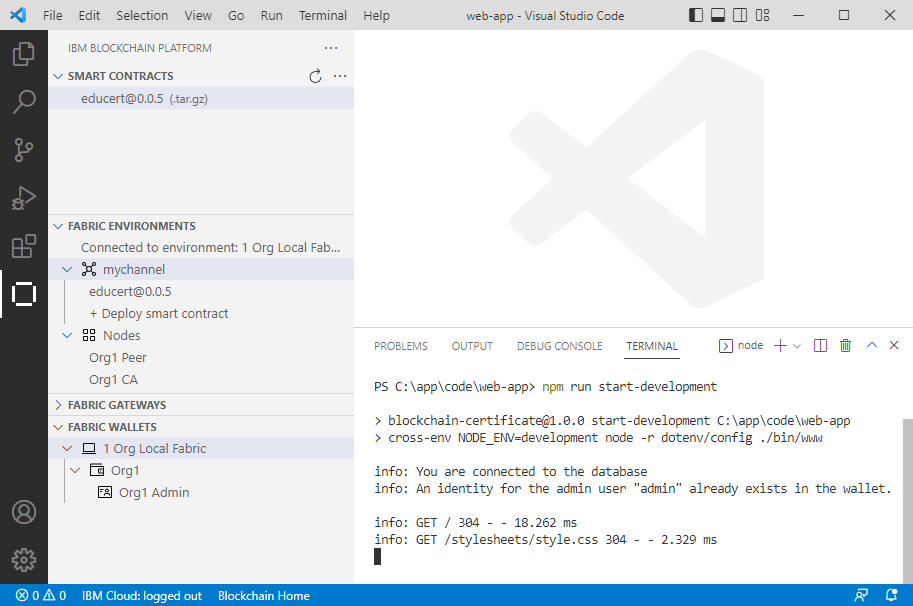
\includegraphics[width=.9\linewidth]{img/ide_start.PNG}
\caption{Chương trình Visual Studio Code}
\label{fig:ide_start}
\end{figure}

\section{Kết quả thực nghiệm}

Sau khi hệ thống quản lý VBCC được khởi động như hình \ref{fig:ide_start}. Giao diện chính có địa chỉ http://localhost:3000/ như hình \ref{fig:main_vbcc}

\begin{figure}[htbp]
\centering
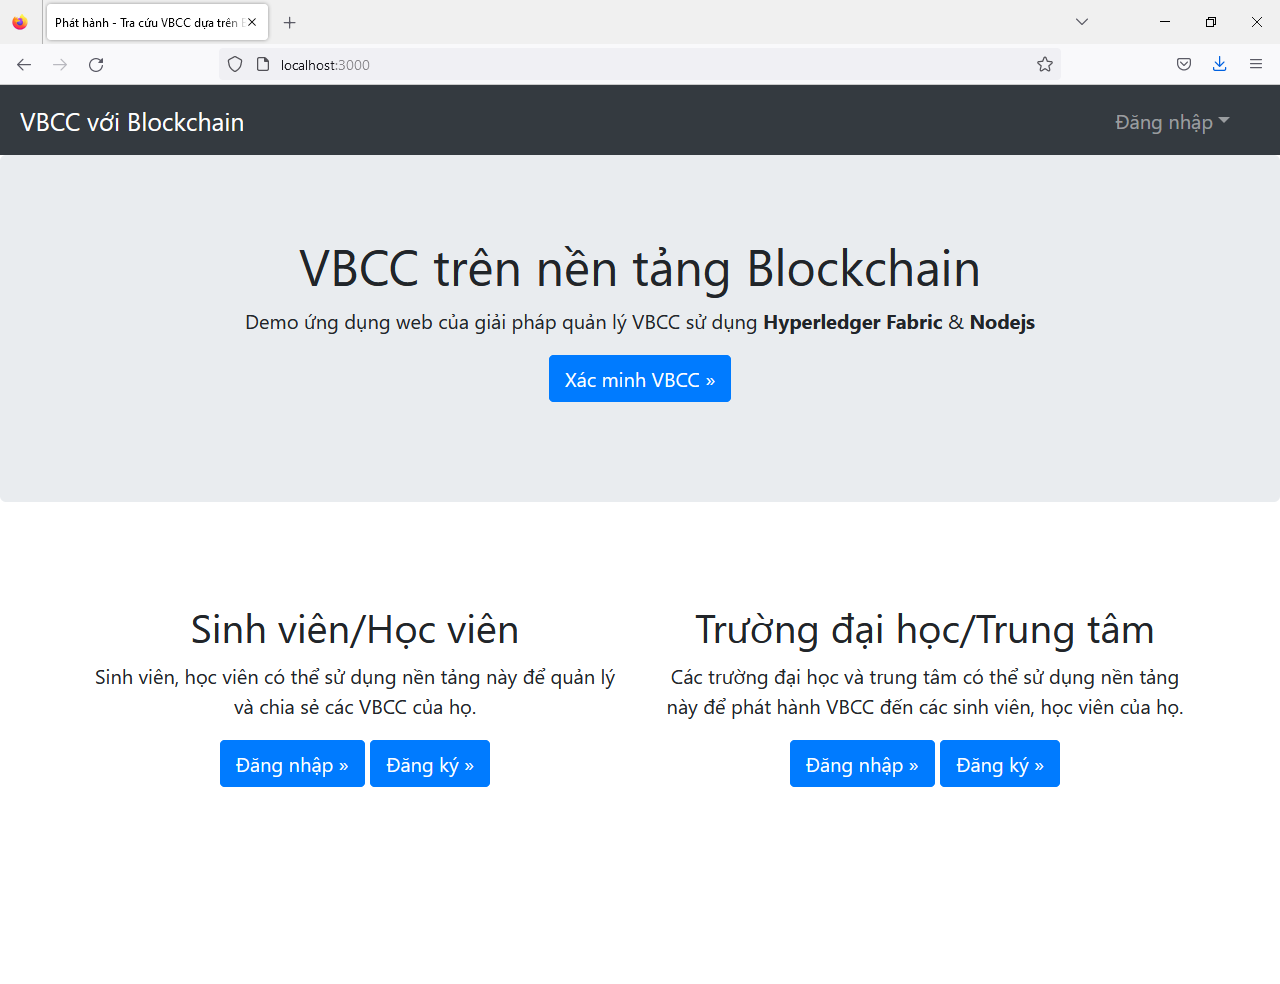
\includegraphics[width=.9\linewidth]{img/main_vbcc.png}
\caption{Giao diện hệ thống}
\label{fig:main_vbcc}
\end{figure}

Quy trình hoạt động của hệ thống được mô trả như hình \ref{fig:vbcc_diagram}

\begin{figure}[htbp]
\centering
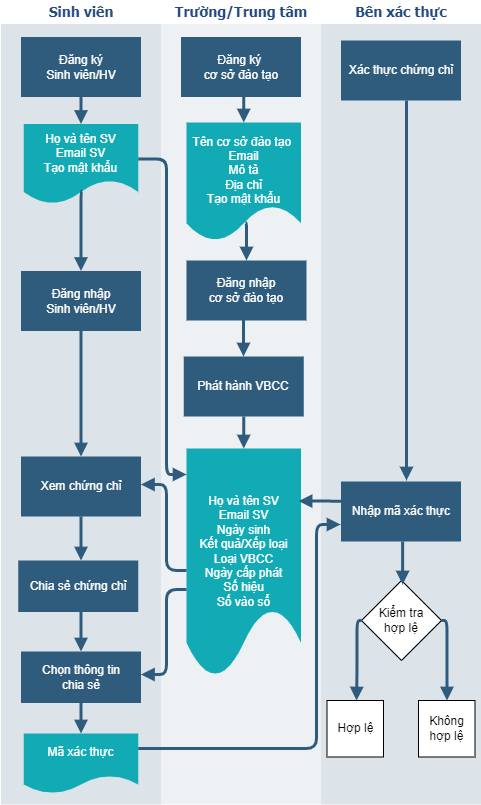
\includegraphics[width=.9\linewidth]{img/vbcc_diagram2.png}
\caption{Quy trình hoạt động của hệ thống}
\label{fig:vbcc_diagram}
\end{figure}

